\chapter{Curvilinear Coordinates}
\label{ch:coordinates}
\begin{chapterintro}
\textbf{You will learn to:} express position, velocity, and acceleration in polar,
cylindrical, and spherical coordinates; differentiate the moving unit vectors; and
recognise the centripetal and Coriolis-like terms that appear in curvilinear
coordinates.
\end{chapterintro}

\section{Polar coordinates}

In the plane, a point $M$ is located by its distance $r$ from the origin and the
angle $\theta$ measured from the $x$-axis. The associated unit vectors are
$\ur$ (radial, pointing away from $O$) and $\ut$ (perpendicular to $\ur$, in the
direction of increasing $\theta$).

\begin{figure}[htbp]
\centering
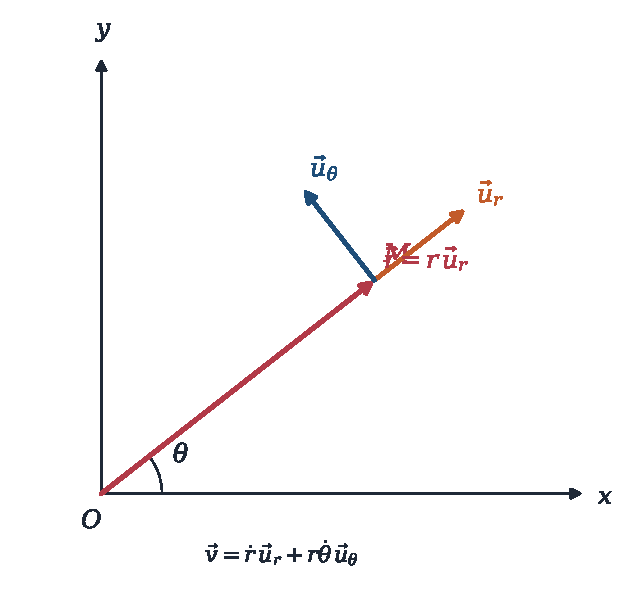
\includegraphics[width=0.66\textwidth]{figures/08_polar_basis.pdf}
\caption{Polar coordinates and the local basis $(\ur,\ut)$. The basis rotates
with the point.}
\label{fig:polar}
\end{figure}

The position vector is simply
\[
\vec r=r\,\ur.
\]
Unlike the Cartesian basis, the polar basis moves:
\[
\frac{\dd\ur}{\dd t}=\dot\theta\,\ut,\qquad
\frac{\dd\ut}{\dd t}=-\dot\theta\,\ur.
\]
Differentiating $\vec r=r\ur$ gives
\[
\vec v=\dot r\,\ur+r\dot\theta\,\ut,
\]
and differentiating again gives
\[
\boxed{\vec a=\left(\ddot r-r\dot\theta^2\right)\ur
+\left(r\ddot\theta+2\dot r\dot\theta\right)\ut.}
\]
The term $-r\dot\theta^2\ur$ is the centripetal acceleration; the term
$2\dot r\dot\theta\,\ut$ is sometimes called the Coriolis term in polar
coordinates.

\begin{keyidea}[Circular motion as a special case]
For a circle, $r=R$ is constant, so $\dot r=\ddot r=0$ and
\[
\vec a=-R\dot\theta^2\,\ur+R\ddot\theta\,\ut
=-\frac{v^2}{R}\ur+a_t\,\ut.
\]
This recovers the centripetal and tangential accelerations of
\cref{ch:plane}.
\end{keyidea}

\section{Cylindrical coordinates}

In three dimensions, cylindrical coordinates $(\rho,\theta,z)$ use the planar
polar coordinates in the $xy$-plane and the Cartesian $z$:
\[
\vec r=\rho\,\vec u_\rho+z\khat.
\]
The velocity and acceleration are
\[
\vec v=\dot\rho\,\vec u_\rho+\rho\dot\theta\,\vec u_\theta+\dot z\,\khat,
\]
\[
\vec a=\left(\ddot\rho-\rho\dot\theta^2\right)\vec u_\rho
+\left(\rho\ddot\theta+2\dot\rho\dot\theta\right)\vec u_\theta
+\ddot z\,\khat.
\]

\section{Spherical coordinates}

Let $r$ be the distance from the origin, $\theta$ the polar angle measured from
the positive $z$-axis, and $\phi$ the azimuthal angle in the $xy$-plane. Then
\[
x=r\sin\theta\cos\phi,\quad
y=r\sin\theta\sin\phi,\quad
z=r\cos\theta.
\]
The position vector is $\vec r=r\,\ur$, and
\[
\vec v=\dot r\,\ur+r\dot\theta\,\ut+r\sin\theta\,\dot\phi\,\uphi.
\]
The acceleration is
\begin{align*}
\vec a={}&\left(\ddot r-r\dot\theta^2-r\sin^2\theta\,\dot\phi^2\right)\ur\\
&+\left(r\ddot\theta+2\dot r\dot\theta-r\sin\theta\cos\theta\,\dot\phi^2\right)\ut\\
&+\left(r\sin\theta\,\ddot\phi+2\dot r\sin\theta\,\dot\phi
+2r\cos\theta\,\dot\theta\dot\phi\right)\uphi.
\end{align*}

\begin{figure}[htbp]
\centering
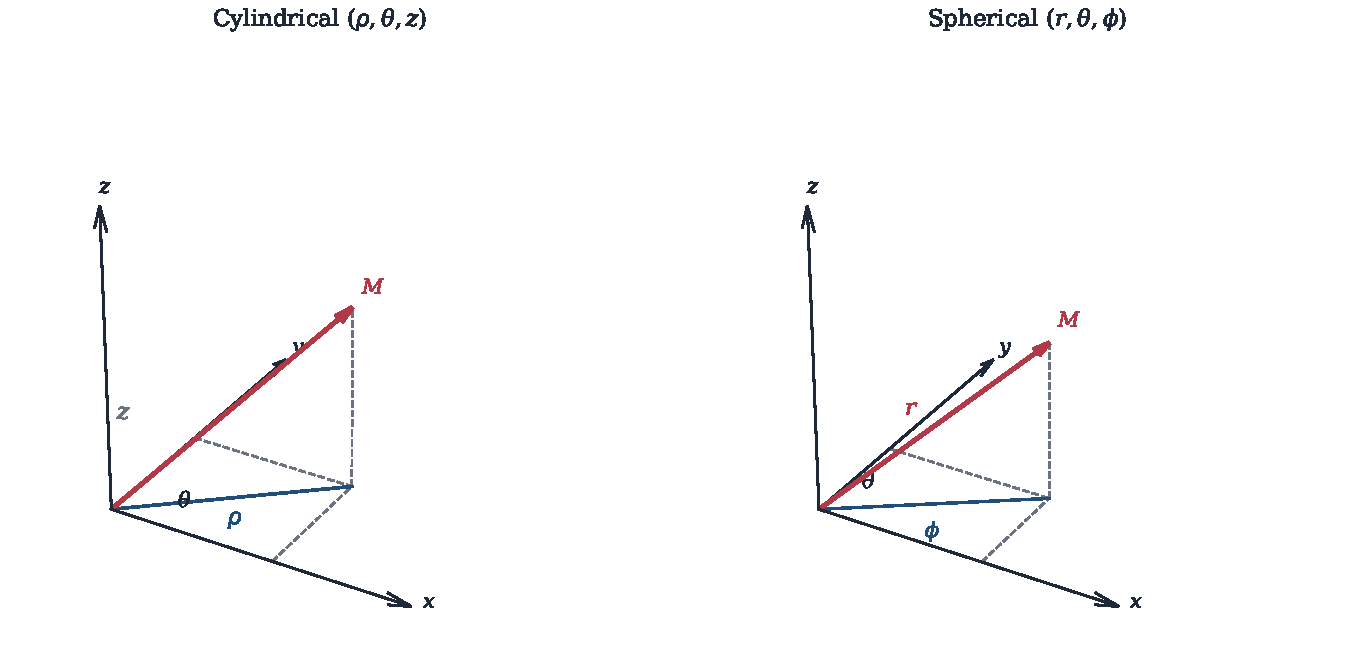
\includegraphics[width=0.98\textwidth]{figures/09_cyl_spherical.pdf}
\caption{Cylindrical coordinates $(\rho,\theta,z)$ and spherical coordinates
$(r,\theta,\phi)$. In the spherical convention used here, $\theta$ is measured
from the $z$-axis.}
\label{fig:cyl-spherical}
\end{figure}

\begin{warning}[Notation varies]
Many books call the azimuthal angle $\theta$ and the polar angle $\phi$. Always
check the definition at the start of a problem. In this book, $\theta$ is the
polar angle from $z$ and $\phi$ is the azimuth in the $xy$-plane.
\end{warning}

\begin{method}[How to use curvilinear coordinates]
\begin{enumerate}[leftmargin=1.5em,itemsep=2pt]
  \item Write down $r(t)$, $\theta(t)$, and (in 3D) $\phi(t)$ or $z(t)$.
  \item Differentiate once to get the general velocity formula.
  \item Differentiate again for acceleration, or use the boxed formulas.
  \item Substitute the time of interest and compute magnitudes with
        $\norm{\vec v}^2=v_r^2+v_\theta^2+v_\phi^2$.
\end{enumerate}
\end{method}

% ===========================================================================
\section{Worked examples}

\begin{worked}[Polar kinematics]
A particle moves in the plane with $r(t)=2t$ (m) and $\theta(t)=t^2$ (rad),
where $t$ is in seconds. Find its velocity and acceleration at
$t=1.00\ \mathrm{s}$.
\end{worked}

\begin{solution}{6.1}
We have
\[
r=2t,\quad \dot r=2,\quad \ddot r=0;\qquad
\theta=t^2,\quad \dot\theta=2t,\quad \ddot\theta=2.
\]
At $t=1$: $r=2$, $\dot r=2$, $\dot\theta=2$, $\ddot\theta=2$, $\ddot r=0$.

Velocity:
\[
\vec v=\dot r\,\ur+r\dot\theta\,\ut
=2\,\ur+2(2)\,\ut=2\,\ur+4\,\ut\ \mathrm{m\,s^{-1}},
\]
\[
v=\sqrt{2^2+4^2}=\sqrt{20}=4.47\ \mathrm{m\,s^{-1}}.
\]
Acceleration:
\[
a_r=\ddot r-r\dot\theta^2=0-2(4)=-8.00\ \mathrm{m\,s^{-2}},
\]
\[
a_\theta=r\ddot\theta+2\dot r\dot\theta=2(2)+2(2)(2)=4+8=12.0\ \mathrm{m\,s^{-2}},
\]
\[
\vec a=-8.00\,\ur+12.0\,\ut\ \mathrm{m\,s^{-2}},\qquad
a=\sqrt{64+144}=14.4\ \mathrm{m\,s^{-2}}.
\]
\end{solution}

\begin{worked}[Motion on a latitude circle]
A particle moves on the sphere of radius $R$ at constant polar angle
$\theta=\pi/3$, with azimuth $\phi=\omega t$. Find its speed and acceleration.
\end{worked}

\begin{solution}{6.2}
Here $r=R$ is constant, $\dot r=\ddot r=0$; $\theta$ is constant, so
$\dot\theta=\ddot\theta=0$; and $\dot\phi=\omega$, $\ddot\phi=0$.

Velocity:
\[
\vec v=r\sin\theta\,\dot\phi\,\uphi
=R\frac{\sqrt3}{2}\omega\,\uphi,
\qquad
v=\frac{\sqrt3}{2}R\omega.
\]
Acceleration:
\[
a_r=-r\sin^2\theta\,\dot\phi^2
=-R\frac34\omega^2,
\]
\[
a_\theta=-r\sin\theta\cos\theta\,\dot\phi^2
=-R\frac{\sqrt3}{2}\frac12\omega^2
=-\frac{\sqrt3}{4}R\omega^2,
\]
\[
a_\phi=0.
\]
Thus
\[
\vec a=-\frac34R\omega^2\,\ur-\frac{\sqrt3}{4}R\omega^2\,\ut,
\qquad
a=\sqrt{\frac{9}{16}+\frac{3}{16}}\,R\omega^2
=\frac{\sqrt3}{2}R\omega^2.
\]
Note that $a=v^2/\rho$, where $\rho=R\sin\theta$ is the radius of the latitude
circle.
\end{solution}

% ===========================================================================
\section{Exercises and Step-by-Step Solutions}

\begin{exercise}{\warm\ Coordinate conversion}
Convert the Cartesian point $(2,-2,3)$ to cylindrical and spherical coordinates.
\end{exercise}

\begin{tabletworkspace}[6.5cm]
\end{tabletworkspace}

\begin{solution}{6.1}
Cylindrical:
\[
\rho=\sqrt{x^2+y^2}=\sqrt{4+4}=\sqrt8=2.83,
\]
\[
\theta=\arctan\frac{y}{x}=\arctan(-1)=-45.0^\circ
\]
(the point is in the fourth quadrant), and $z=3.00$.

Spherical:
\[
r=\sqrt{x^2+y^2+z^2}=\sqrt{4+4+9}=\sqrt{17}=4.12,
\]
\[
\theta=\arccos\frac{z}{r}=\arccos\frac{3}{4.12}=43.3^\circ,
\]
and $\phi=-45.0^\circ$.
\end{solution}

\begin{exercise}{\warm\ Uniform circular motion in polar form}
A particle moves on a circle of radius $3.00\ \mathrm{m}$ with
$\theta(t)=2.00t$ rad. Find its velocity and acceleration at
$t=1.00\ \mathrm{s}$ using polar coordinates.
\end{exercise}

\begin{tabletworkspace}[6.5cm]
\end{tabletworkspace}

\begin{solution}{6.2}
With $r=R=3.00$ constant, $\dot r=\ddot r=0$, and
$\dot\theta=2.00$, $\ddot\theta=0$:
\[
\vec v=R\dot\theta\,\ut=3.00(2.00)\,\ut=6.00\,\ut\ \mathrm{m\,s^{-1}},
\]
\[
v=6.00\ \mathrm{m\,s^{-1}}.
\]
\[
a_r=-R\dot\theta^2=-3.00(4.00)=-12.0\ \mathrm{m\,s^{-2}},
\]
\[
a_\theta=R\ddot\theta=0.
\]
Thus
\[
\vec a=-12.0\,\ur\ \mathrm{m\,s^{-2}},
\qquad a=12.0\ \mathrm{m\,s^{-2}}
\]
toward the centre.
\end{solution}

\begin{exercise}{\warm\ Polar kinematics}
A particle has $r(t)=t^2$ (m) and $\theta(t)=t$ (rad). Find $\vec v$ and
$\vec a$ at $t=2.00\ \mathrm{s}$, and their magnitudes.
\end{exercise}

\begin{tabletworkspace}[6.5cm]
\end{tabletworkspace}

\begin{solution}{6.3}
\[
r=t^2\implies \dot r=2t,\ \ddot r=2;\qquad
\theta=t\implies \dot\theta=1,\ \ddot\theta=0.
\]
At $t=2$: $r=4$, $\dot r=4$, $\dot\theta=1$.

\[
\vec v=4\,\ur+4(1)\,\ut=4\,\ur+4\,\ut\ \mathrm{m\,s^{-1}},
\qquad v=4\sqrt2=5.66\ \mathrm{m\,s^{-1}}.
\]
\[
a_r=\ddot r-r\dot\theta^2=2-4(1)=-2.00\ \mathrm{m\,s^{-2}},
\]
\[
a_\theta=r\ddot\theta+2\dot r\dot\theta=0+2(4)(1)=8.00\ \mathrm{m\,s^{-2}}.
\]
\[
\vec a=-2.00\,\ur+8.00\,\ut\ \mathrm{m\,s^{-2}},
\qquad a=\sqrt{4+64}=8.25\ \mathrm{m\,s^{-2}}.
\]
\end{solution}

\begin{exercise}{\core\ Radial oscillation}
A particle moves with $r(t)=2+\cos t$ (m) and $\theta(t)=t$ (rad). Find
$\vec v$ and $\vec a$ at $t=\pi/2$.
\end{exercise}

\begin{tabletworkspace}[6.5cm]
\end{tabletworkspace}

\begin{solution}{6.4}
\[
r=2+\cos t\implies \dot r=-\sin t,\ \ddot r=-\cos t.
\]
At $t=\pi/2$: $r=2$, $\dot r=-1$, $\ddot r=0$; and $\theta=t$ gives
$\dot\theta=1$, $\ddot\theta=0$.

\[
\vec v=\dot r\,\ur+r\dot\theta\,\ut=-\ur+2\ut\ \mathrm{m\,s^{-1}},
\qquad v=\sqrt{1+4}=\sqrt5=2.24\ \mathrm{m\,s^{-1}}.
\]
\[
a_r=\ddot r-r\dot\theta^2=0-2(1)=-2.00\ \mathrm{m\,s^{-2}},
\]
\[
a_\theta=r\ddot\theta+2\dot r\dot\theta=0+2(-1)(1)=-2.00\ \mathrm{m\,s^{-2}}.
\]
\[
\vec a=-2.00\,\ur-2.00\,\ut\ \mathrm{m\,s^{-2}},
\qquad a=\sqrt{8}=2.83\ \mathrm{m\,s^{-2}}.
\]
\end{solution}

\begin{exercise}{\core\ Cylindrical motion}
A particle has $\rho=2.00\ \mathrm{m}$ (constant), $\theta=3.00t$ rad, and
$z=4.00t^2$ m. Find its velocity and acceleration at $t=1.00\ \mathrm{s}$.
\end{exercise}

\begin{tabletworkspace}[6.5cm]
\end{tabletworkspace}

\begin{solution}{6.5}
\[
\rho=2,\ \dot\rho=0,\ \ddot\rho=0;\qquad
\theta=3t,\ \dot\theta=3,\ \ddot\theta=0;\qquad
z=4t^2,\ \dot z=8t,\ \ddot z=8.
\]
At $t=1$: $\dot z=8.00$, $\ddot z=8.00$.

\[
\vec v=\rho\dot\theta\,\vec u_\theta+\dot z\,\khat
=2(3)\vec u_\theta+8\khat=6.00\,\vec u_\theta+8.00\,\khat\ \mathrm{m\,s^{-1}},
\]
\[
v=\sqrt{36+64}=10.0\ \mathrm{m\,s^{-1}}.
\]
\[
a_\rho=-\rho\dot\theta^2=-2(9)=-18.0\ \mathrm{m\,s^{-2}},
\]
\[
a_\theta=\rho\ddot\theta+2\dot\rho\dot\theta=0,
\]
\[
a_z=\ddot z=8.00\ \mathrm{m\,s^{-2}}.
\]
\[
\vec a=-18.0\,\vec u_\rho+8.00\,\khat\ \mathrm{m\,s^{-2}},
\qquad a=\sqrt{324+64}=19.7\ \mathrm{m\,s^{-2}}.
\]
\end{solution}

\begin{exercise}{\core\ Motion on the equator}
A particle moves on the equator of a sphere of radius $R$ with azimuth
$\phi=\omega t$. Use spherical coordinates to find its speed and acceleration.
\end{exercise}

\begin{tabletworkspace}[6.5cm]
\end{tabletworkspace}

\begin{solution}{6.6}
On the equator, $\theta=\pi/2$ is constant, so
$\dot\theta=\ddot\theta=0$, and $r=R$ is constant. With $\dot\phi=\omega$,
\[
\vec v=R\sin\frac{\pi}{2}\,\omega\,\uphi=R\omega\,\uphi,
\qquad v=R\omega.
\]
The acceleration components are
\[
a_r=-R\sin^2\frac{\pi}{2}\,\omega^2=-R\omega^2,
\]
\[
a_\theta=-R\sin\frac{\pi}{2}\cos\frac{\pi}{2}\,\omega^2=0,
\qquad a_\phi=0.
\]
Thus
\[
\vec a=-R\omega^2\,\ur,
\]
which is the familiar centripetal acceleration toward the centre of the sphere.
\end{solution}

\begin{exercise}{\core\ Derivatives of the polar basis}
Starting from
$\ur=\cos\theta\,\ihat+\sin\theta\,\jhat$ and
$\ut=-\sin\theta\,\ihat+\cos\theta\,\jhat$, prove that
\[
\frac{\dd\ur}{\dd t}=\dot\theta\,\ut,\qquad
\frac{\dd\ut}{\dd t}=-\dot\theta\,\ur.
\]
\end{exercise}

\begin{tabletworkspace}[6.5cm]
\end{tabletworkspace}

\begin{solution}{6.7}
Differentiate $\ur$:
\[
\frac{\dd\ur}{\dd t}
=-\sin\theta\,\dot\theta\,\ihat+\cos\theta\,\dot\theta\,\jhat
=\dot\theta(-\sin\theta\,\ihat+\cos\theta\,\jhat)
=\dot\theta\,\ut.
\]
Similarly,
\[
\frac{\dd\ut}{\dd t}
=-\cos\theta\,\dot\theta\,\ihat-\sin\theta\,\dot\theta\,\jhat
=-\dot\theta(\cos\theta\,\ihat+\sin\theta\,\jhat)
=-\dot\theta\,\ur.
\]
\end{solution}

\begin{exercise}{\core\ Circular motion from the general formula}
Starting from the general polar acceleration, set $r=R=$ constant and recover
\[
\vec a=-\frac{v^2}{R}\ur+a_t\,\ut.
\]
Identify $v$ and $a_t$ in terms of $\theta$.
\end{exercise}

\begin{tabletworkspace}[6.5cm]
\end{tabletworkspace}

\begin{solution}{6.8}
For $r=R$, $\dot r=\ddot r=0$. The general formulas give
\[
\vec a=-R\dot\theta^2\,\ur+R\ddot\theta\,\ut.
\]
The speed is $v=R\dot\theta$, so
\[
R\dot\theta^2=\frac{(R\dot\theta)^2}{R}=\frac{v^2}{R}.
\]
The tangential acceleration is
\[
a_t=\frac{\dd v}{\dd t}=R\ddot\theta.
\]
Hence
\[
\vec a=-\frac{v^2}{R}\ur+R\ddot\theta\,\ut
=-\frac{v^2}{R}\ur+a_t\,\ut.
\]
\end{solution}

\begin{exercise}{\mastery\ Conservation of areal velocity}
For a central force the transverse acceleration vanishes: $a_\theta=0$. Show
that this implies
\[
r^2\dot\theta=\text{constant}.
\]
Interpret this constant geometrically as twice the areal velocity.
\end{exercise}

\begin{tabletworkspace}[6.5cm]
\end{tabletworkspace}

\begin{solution}{6.9}
The transverse acceleration is
\[
a_\theta=r\ddot\theta+2\dot r\dot\theta
=\frac1r\frac{\dd}{\dd t}\left(r^2\dot\theta\right).
\]
If $a_\theta=0$, then
\[
\frac{\dd}{\dd t}\left(r^2\dot\theta\right)=0
\implies
r^2\dot\theta=h=\text{constant}.
\]
In polar coordinates the area swept by the radius vector in time $\dd t$ is
\[
\dd A=\frac12r^2\,\dd\theta,
\]
so the areal velocity is
\[
\frac{\dd A}{\dd t}=\frac12r^2\dot\theta=\frac h2,
\]
which is constant. This is Kepler's second law.
\end{solution}

\begin{exercise}{\mastery\ Logarithmic spiral}
A particle moves with $r(t)=ae^{bt}$ and $\theta(t)=ct$, where $a,b,c$ are
constants. Find the radial and transverse components of velocity and
acceleration. Show that the acceleration makes a constant angle with the radial
direction.
\end{exercise}

\begin{tabletworkspace}[6.5cm]
\end{tabletworkspace}

\begin{solution}{6.10}
With $r=ae^{bt}$,
\[
\dot r=ab\,e^{bt},\qquad \ddot r=ab^2e^{bt},
\]
and with $\theta=ct$, $\dot\theta=c$, $\ddot\theta=0$. Therefore
\[
v_r=\dot r=ab\,e^{bt},\qquad
v_\theta=r\dot\theta=ac\,e^{bt},
\]
so
\[
\vec v=ae^{bt}\left(b\,\ur+c\,\ut\right).
\]
For the acceleration,
\[
a_r=\ddot r-r\dot\theta^2
=ae^{bt}\left(b^2-c^2\right),
\]
\[
a_\theta=r\ddot\theta+2\dot r\dot\theta
=2abc\,e^{bt}.
\]
Thus
\[
\vec a=ae^{bt}\left[(b^2-c^2)\,\ur+2bc\,\ut\right].
\]
The ratio $a_\theta/a_r=2bc/(b^2-c^2)$ is independent of time, so the acceleration
makes a constant angle with the radial direction. The curve is a logarithmic
spiral.
\end{solution}

